\section{Design and Implementation}

\subsection{System Overview}
\begin{figure}[h]
	\centering
  	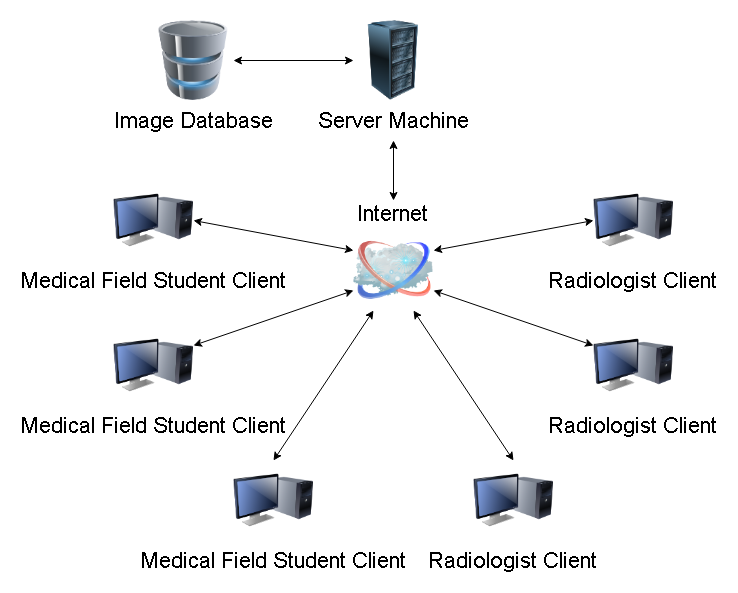
\includegraphics[scale=0.5]{images/systemOverview.png}
	 \caption{System Overview, Mammo}
  	\label{fig:systemOverview}
\end{figure}

	The Decision Support System includes a typical client-server architecture. The client sends requests to the server. The server processes the client's request. There are two types of clients namely the Medical Field Student Client (MFSC) and the Radiologist Client (RC). The MFSC and the RC can send mammogram images through desktop computers for evaluation to the server by which the server, in turn, returns the results. The MFSC may also request for an exam, and the server redirects the MFSC to the exam proper.
\clearpage

\subsection{Use Case Diagram}
\qquad Figure \ref{fig:useCase} shows the general functionalities of each user. Both the Medical Field Student and Radiologist have the functionality of uploading a mammogram image for the system to classify whether benign or malignant, and retrieving the classification result. The Medical Field Student also has the option to take an exam on screening mammograms.

\begin{figure}[!htb]
	\centering
  	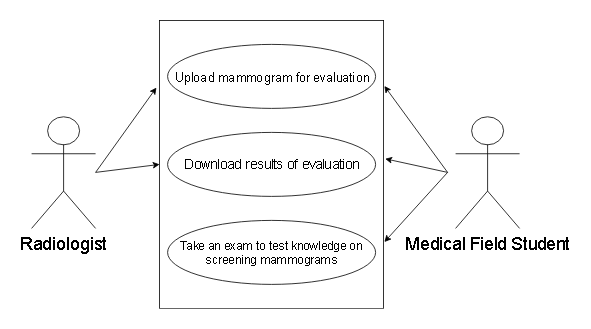
\includegraphics[scale=0.8]{images/useCase.png}
	 \caption{Use Case Diagram, Mammo}
  	\label{fig:useCase}
\end{figure}
\clearpage


\subsection{Activity Diagram}

\begin{enumerate}
	\item{Radiologist} \\
	The radiologist can also send a mammgram image for evaluation using the web application.

\begin{figure}[h]
	\centering
  	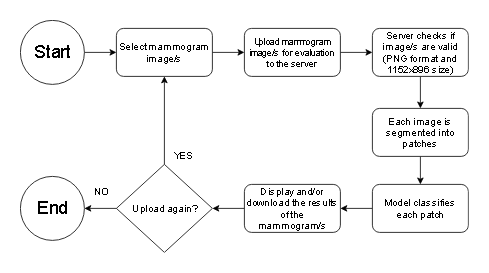
\includegraphics[scale=0.75]{images/radiologist.png}
	 \caption{Radiologist Activity Diagram, Mammo}
  	\label{fig:radiologist}
\end{figure}
\clearpage

	\item{Medical Field Student} \\
	The medical field student can send a mammogram image for evaluation using the web application. The medical field student may also request for an exam on screening mammograms. The results of the exam are given immediately after.

\begin{figure}[h]
	\centering
  	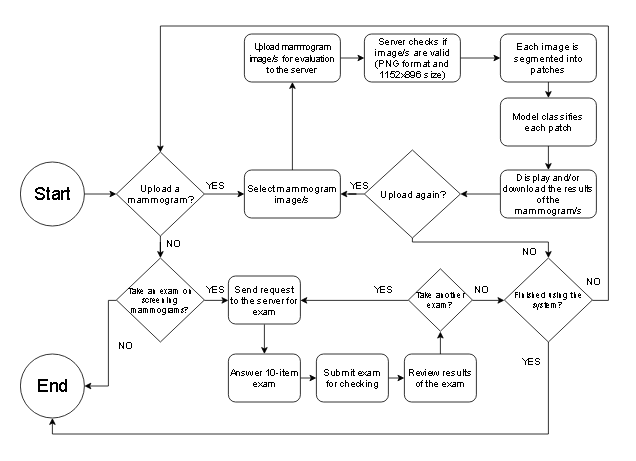
\includegraphics[scale=0.75]{images/medicalFieldStudent.png}
	 \caption{Medical Field Student Activity Diagram, Mammo}
  	\label{fig:medicalFieldStudent}
\end{figure}
\end{enumerate}
\clearpage

\subsection{Technical Architecture}
\qquad The recommended requirements for the server machine include:

\begin{itemize}
	\item 2 GHz CPU rate or higher
	\item Graphics Processing Unit (GPU) specifically a NVIDIA Graphics Card with 3.0 compute capability or higher
	\item 8 GB RAM or higher
	\item Up to 2 GB of free disk space
\end{itemize}

	The client side must have any of the following compatible up-to-date web browsers:

\begin{itemize}
	\item Google Chrome
	\item Mozilla Firefox
	\item Safari
\end{itemize}

\subsection{Data Set}
\qquad The data set used is the CBIS-DDSM (Curated Breast Imaging Subset of the Digital Database for Screening Mammography) which is an updated and standardized version of the DDSM \cite{CBIS-DDSM}. The data set contains 2583 cropped mammogram ROI images in DICOM format of 1249 patients labeled as benign or malignant cases with verified pathology information. It includes the CC and MLO views for most of the screened breasts. The data set is publicly available through TCIA (The Cancer Imaging Archive) which is an online service that hosts a large archive of medical images of cancer accessible for public download \cite{TCIA}.